\documentclass[final,hyperref={pdfpagelabels=false}]{beamer}

\mode<presentation>{\usetheme{I6pd2_hugo}}
\usepackage[english]{babel}
\usepackage[utf8]{inputenc}
\usepackage{amsmath,amsthm, amssymb, latexsym, subfigure, graphicx,array,booktabs,tabularx, caption}
%\usepackage{times}\usefonttheme{professionalfonts}  % obsolete
%\usefonttheme[onlymath]{serif}
\boldmath
\usepackage[orientation=portrait,size=a0,scale=1.4,debug]{beamerposter}
% change list indention level
% \setdefaultleftmargin{3em}{}{}{}{}{}
\usecaptiontemplate{
\small
\structure{\insertcaptionname~\insertcaptionnumber:}
\insertcaption
}


%\usepackage{snapshot} % will write a .dep file with all dependencies, allows for easy bundling

\newcolumntype{Z}{>{\centering\arraybackslash}X} % centered tabularx columns
\newcommand{\pphantom}{\textcolor{ta3aluminium}} % phantom introduces a vertical space in p formatted table columns??!!

\listfiles

%%%%%%%%%%%%%%%%%%%%%%%%%%%%%%%%%%%%%%%%%%%%%%%%%%%%%%%%%%%%%%%%%%%%%%%%%%%%%%%%%%%%%%

\title{Impedance Studies of the LHC Injection Kicker Magnets for HL-LHC}
\author{H. Day, M.J. Barnes, L. Coralejo Feliciano}
\institute[CERN]{CERN, Geneva, Switzerland}
\date[May 2015]{May 2015}

%%%%%%%%%%%%%%%%%%%%%%%%%%%%%%%%%%%%%%%%%%%%%%%%%%%%%%%%%%%%%%%%%%%%%%%%%%%%%%%%%%%%%%
\newlength{\columnheight}
\setlength{\columnheight}{105cm}


%%%%%%%%%%%%%%%%%%%%%%%%%%%%%%%%%%%%%%%%%%%%%%%%%%%%%%%%%%%%%%%%%%%%%%%%%%%%%%%%%%%%%%
\begin{document}
\begin{frame}
  \begin{columns}
    % ---------------------------------------------------------%
    % Set up a column 
    \begin{column}{.49\textwidth}
      \begin{beamercolorbox}[center,wd=\textwidth]{postercolumn}
        \begin{minipage}[T]{.95\textwidth}  % tweaks the width, makes a new \textwidth
          \parbox[t][\columnheight]{\textwidth}{ % must be some better way to set the the height, width and textwidth simultaneously
            % Since all columns are the same length, it is all nice and tidy.  You have to get the height empirically
            % ---------------------------------------------------------%
            % fill each column with content            
            \begin{block}{Summary}
\small{
The LHC injection kicker magnets (MKIs) experienced strong heating during the first operational run, identified as being caused by power loss due to wakefields induced by circulating beam. Studies of the beam coupling impedance of the beam screen, a series of conductors embedded in a ceramic tube placed in the aperture of the ferrite yoke to screen the ferrite from the beam, resulted in new design offering improved screening: this is predicted to reduce the heating to acceptable levels for operation with 25ns beam during run 2 of the LHC. However higher beam intensities proposed for HL-LHC operation are predicted to again cause strong heating to occur. Further studies have been carried out to reduce the beam induced power loss by optimising the beam screen design, some key results and findings of which are presented here.
}
\end{block}
            \vfill
	\begin{block}{Background}
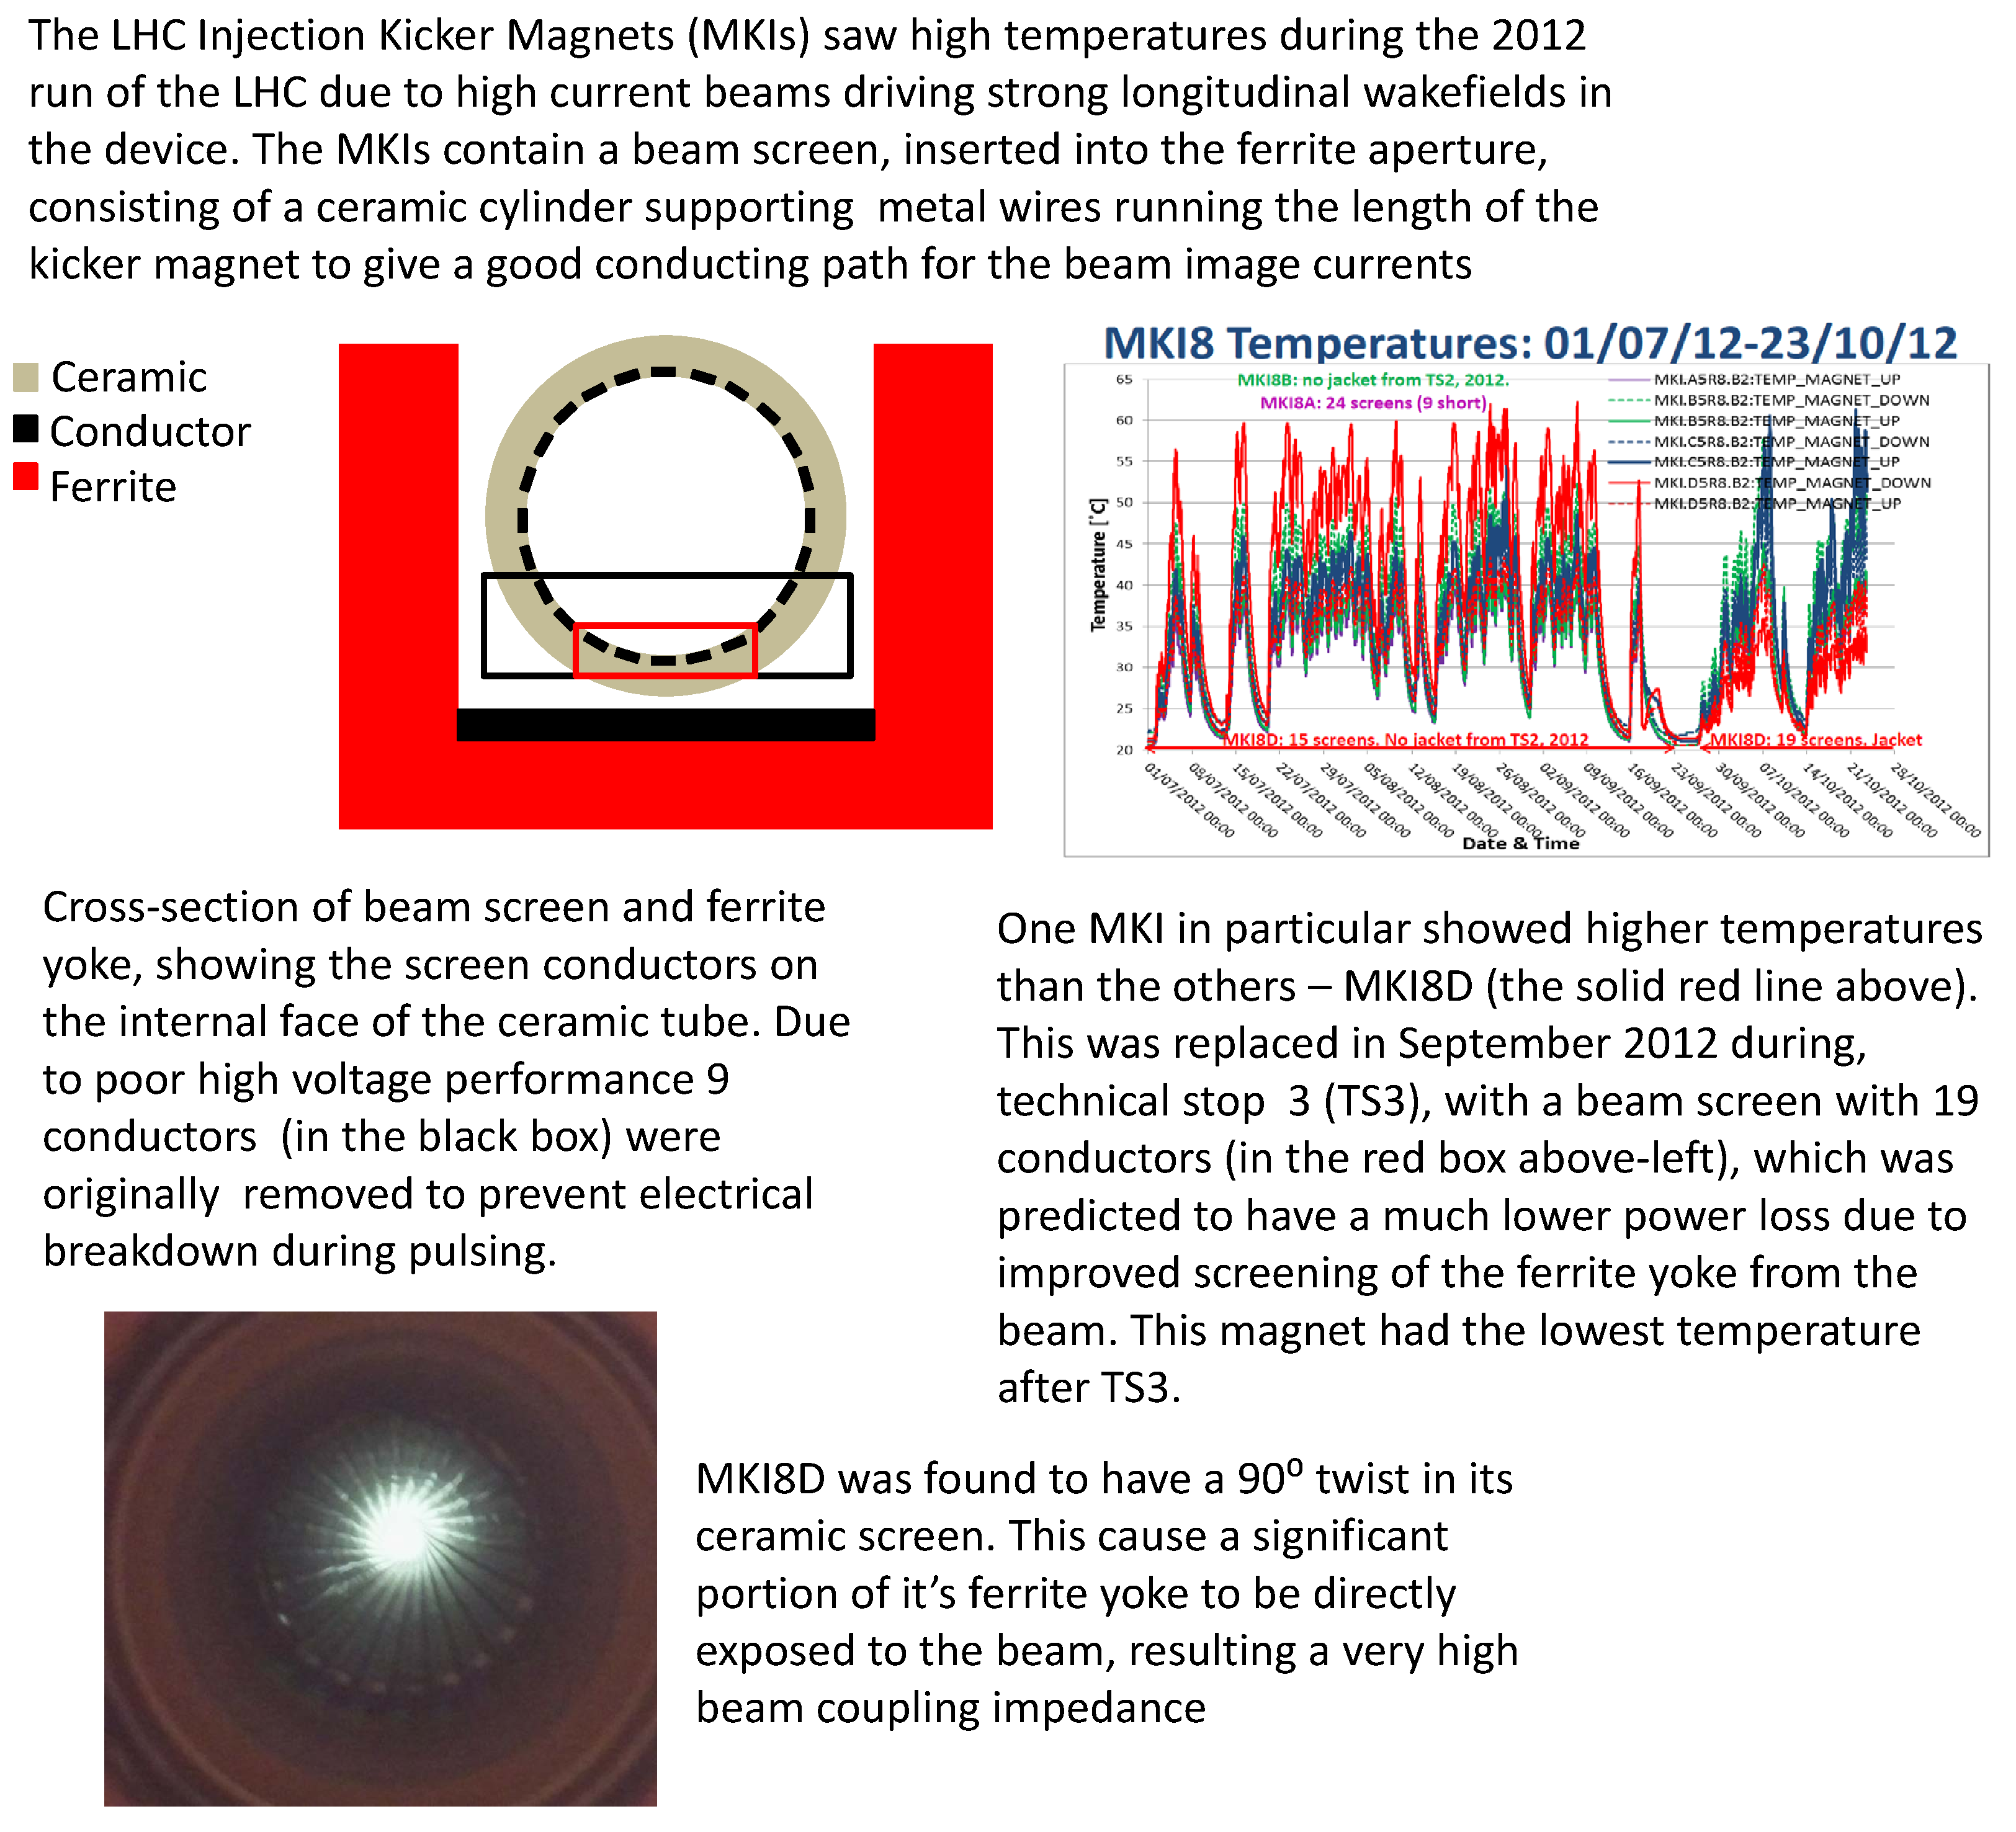
\includegraphics[width=1.0\textwidth]{introductionPicture.pdf}
	\end{block}
 \vfill
	\begin{block}{Beam Screen}
\begin{figure}
\subfigure[]{
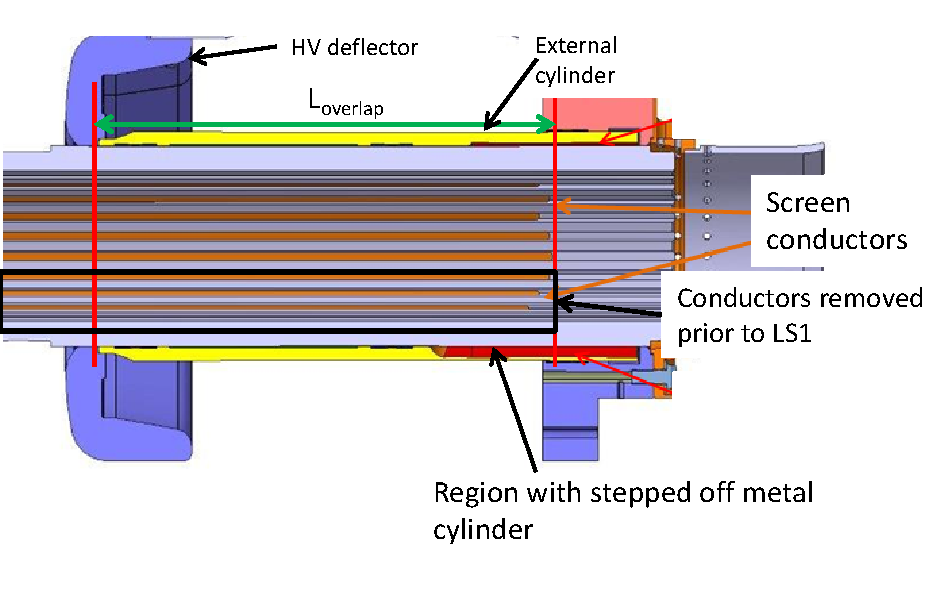
\includegraphics[width=0.55\textwidth]{beamScreenCrossSectionLabelled.pdf}
}\subfigure[]{
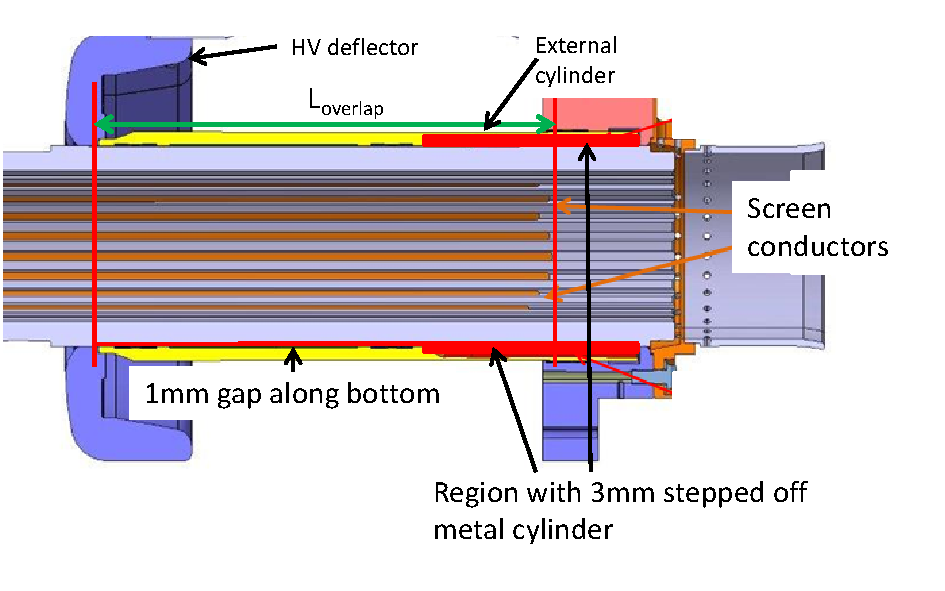
\includegraphics[width=0.55\textwidth]{HLLHCLayout.pdf}
}\end{figure}

\begin{itemize}
\item{The beam screen design installed in the MKIs during long shutdown 1 (LS1) [1], has been designed to permit the inclusion of 24 screen conductors in the ceramic tube, whilst lowering the surface electric field on the ceramic tube during kicker pulsing to reduce the chance of surface flashover.}
\item{The capacitively coupled end is significantly changed:}
\begin{itemize}
\item{The external metallization is replaced by an external metal tube which steps away from the ceramic tube near the ends of the screen conductors. This reduces the surface electric field on the ceramic tube significantly. Tapering the length of the conductors also helps this reduction.}
\item{This allows 24 screen conductors to be placed back in the beam screen, greatly improving the screening of the ferrite yoke from the beam. [2]}
\end{itemize}
\item{A revised beam screen is suggested for HL-LHC:}
\begin{itemize}
\item{The external metal tube is modified to include a 1mm air gap at the HV plate side of the tube for the whole length of the tube, tapering to a 0mm gap across a 90$^{\circ}$ arc at the top of the tube on the ground plate side to reduce the likelihood of surface flashover.}
\item{The total overlap between the screen conductors in decreased to increase the frequency of any resonances associated with this area [2]}
\end{itemize}
\end{itemize}

	\end{block}

            \vfill


         \vfill
          }
        \end{minipage}
      \end{beamercolorbox}
    \end{column}
    % ---------------------------------------------------------%
    % end the column

    % ---------------------------------------------------------%
    % Set up a column 
    \begin{column}{.49\textwidth}
      \begin{beamercolorbox}[center,wd=\textwidth]{postercolumn}
        \begin{minipage}[T]{.95\textwidth} % tweaks the width, makes a new \textwidth
          \parbox[t][\columnheight]{\textwidth}{ % must be some better way to set the the height, width and textwidth simultaneously
            % Since all columns are the same length, it is all nice and tidy.  You have to get the height empirically
            % ---------------------------------------------------------%
            % fill each column with content
\begin{block}{Impedance Characteristics of the New Design}
\begin{itemize}
\begin{small}
\item{Previous work [2] has shown that the resonant frequency, $f_{res}$, of the beam impedance is determined by the length of the overlap between the screen conductors and the external metal cylinder, given by:}
\begin{equation}
f_{res} = \frac{n c}{2 \sqrt{\epsilon_{r}}\left( L_{overlap} + \delta_{fringe} \right)}
\end{equation}
where $n$ is an integer, $c$ the speed of light, $\epsilon_{r}$ is the relative permitivitty of the ceramic tube, $L_{overlap}$ the length of overlap between the screen conductors and the external cylinder and $\delta_{fringe}$ the influence of the fringe fields on the effective length.
\item{The beam current spectrum decreases at high frequencies, implying that the power loss (Eqn.~\ref{eqn:powLoss}) can be reduced by increasing the resonant frequencies.}
\begin{equation}
P_{loss} = 2 \left( f_{0} e M  N_{b}\right)^{2} \displaystyle\sum\limits_{n = -\infty}^{\infty}  \left| \lambda \left( p M \omega_{0} \right)  \right|^{2} \Re{}e \left[ Z_{\parallel} \left( p M \omega_{0} \right) \right]
\label{eqn:powLoss}
\end{equation}
where $f_{0}$ is the revolution frequnecy, $\omega_{0} = 2\pi f_{0}$, $e$ is the charge of an electron, $N_{b}$ is the number of particles per bunch, $M$ is the number of bunches in the machine, $\lambda (\omega)$ is the beam current spectrum, and $\Re{}e(Z_{\parallel}(\omega))$ is the real component of the longitudinal beam coupling impedance.
\item{The effect of the small air gap in the proposed new design also needs to be verified}
\end{small}
\end{itemize}


\begin{figure}
\subfigure[]{
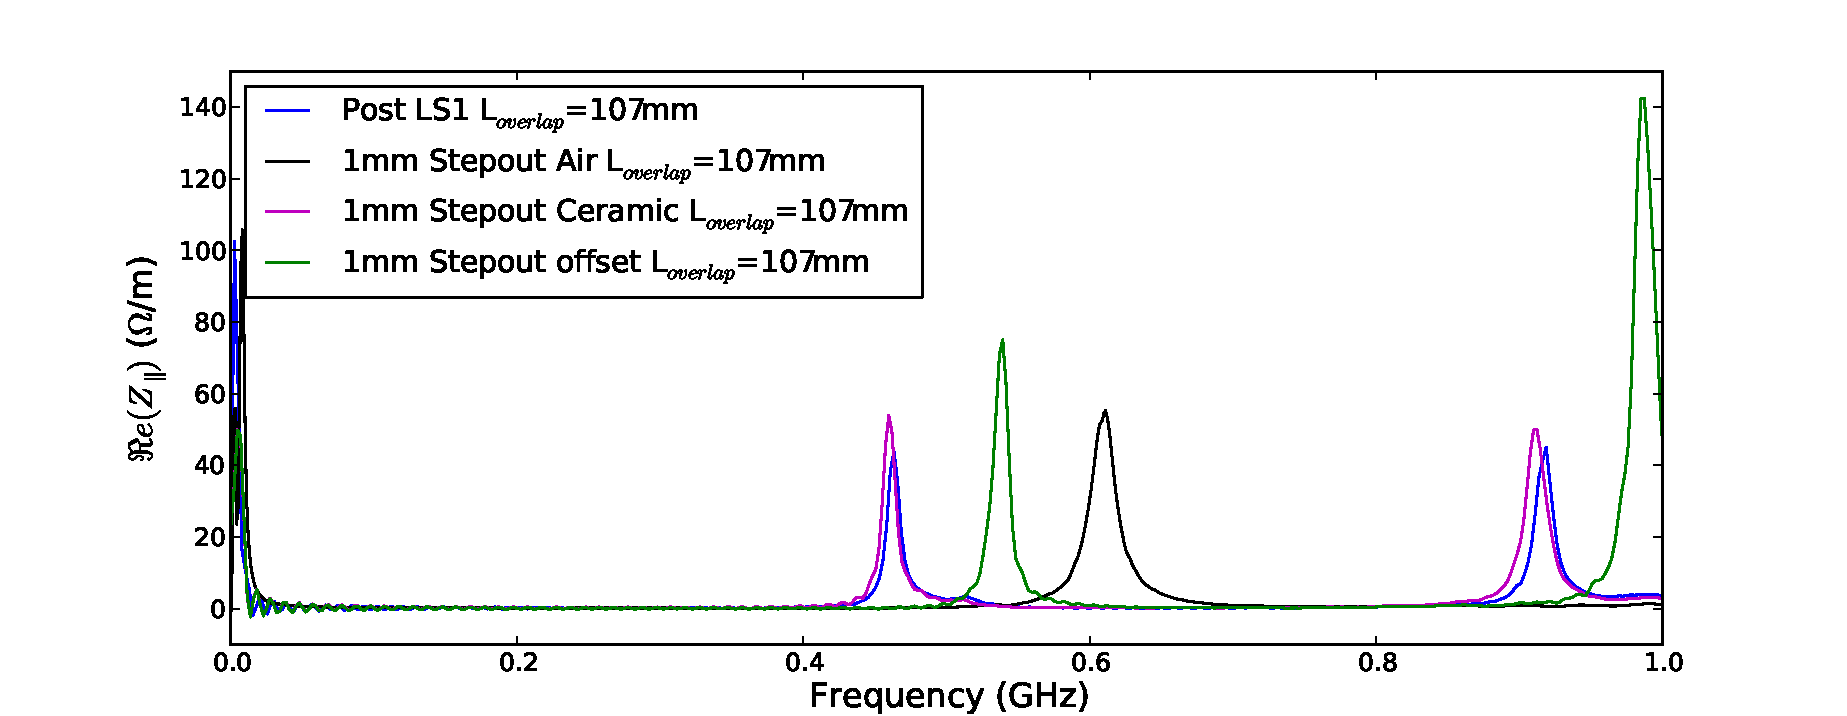
\includegraphics[width=0.4\textwidth]{differentScreenSpacings.pdf}
\label{fig:differentEndArrangement}}
\subfigure[]{
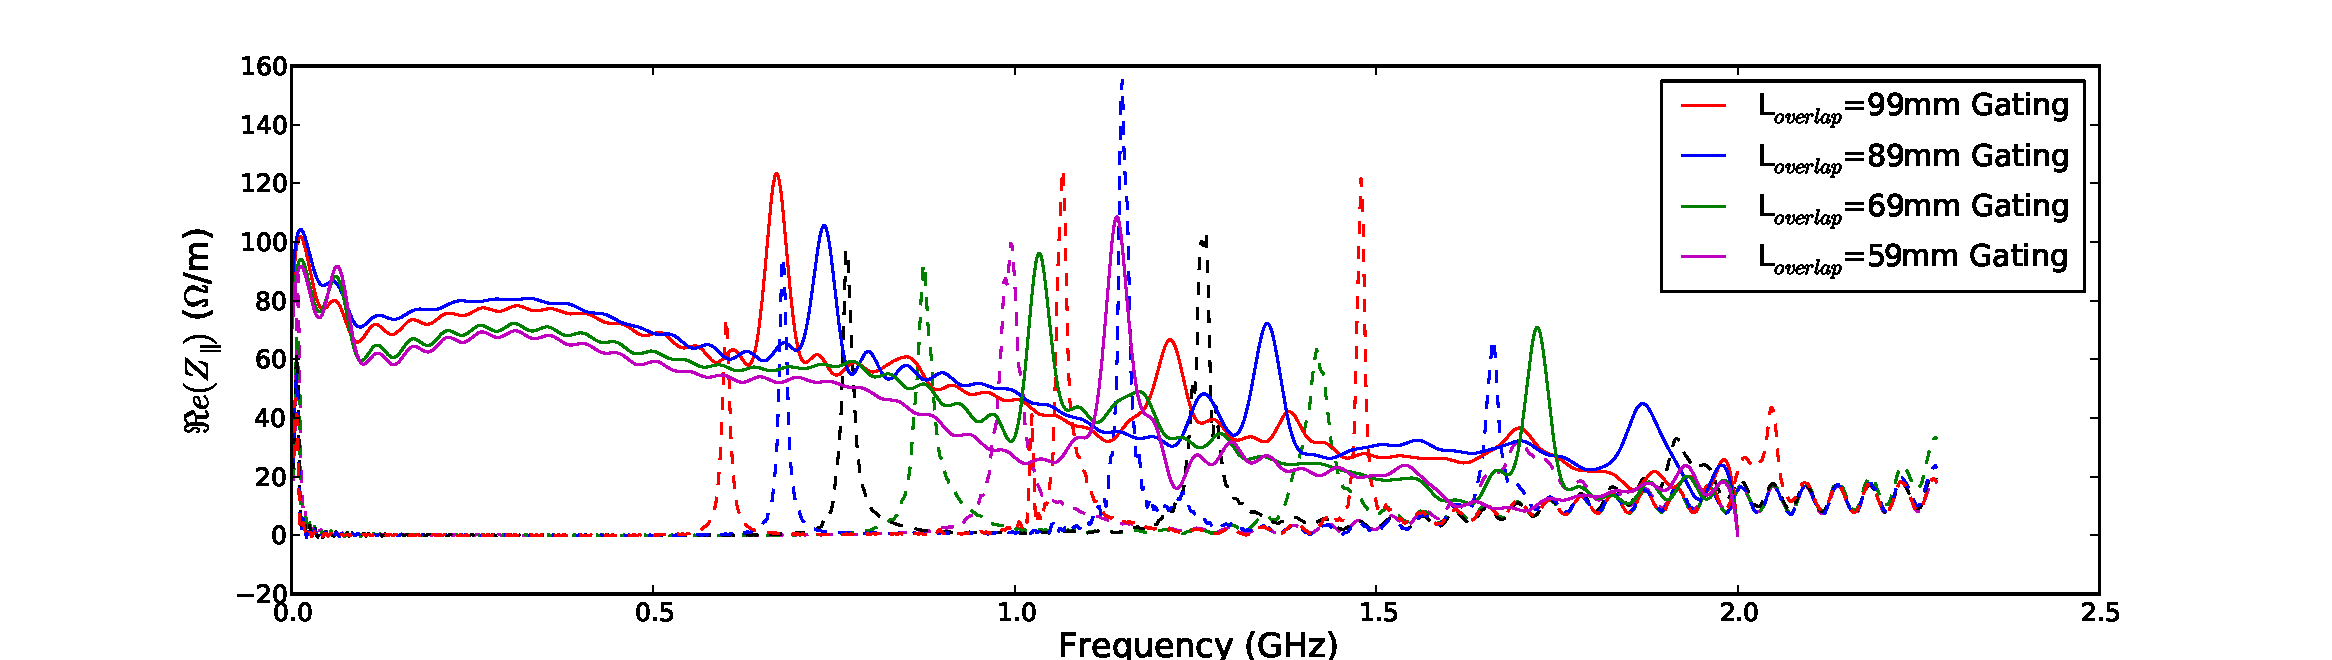
\includegraphics[width=0.55\textwidth]{simMeasGatingOverlap.pdf}
\label{fig:simMeasComp}}
\end{figure}

\begin{itemize}
\item{Simulations of small air gap were carried out using CST Particle Studio for the following cases, each with $L_{overlap}$=107mm: a) as the post-LS1 setup, b) a 1mm air-gap between the tube and the external cylinder, c) as for (b) but the air is replaced by ceramic, d) an offset air-gap, resulting in a gap of 1mm at the bottom and 0mm at the top. The results are shown in Fig.~\ref{fig:differentEndArrangement}. It was found that the proposed gap increased the resonant frequency for the same length (due to decreased capacitance) - a beneficial result}
\item{Simulations and measurements of different values of $L_{overlap}$ were carried out; the measurements were made using the resonant coaxial wire method and the classical coaxial wire method (without matching resistor network, but with time domain gating)}
\item{Results for the simulations (dashed lines) and classical wire measurements (solid lines) are shown in Fig.~\ref{fig:simMeasComp} - in both the simulations and measurements $f_{res}$ is seen to increase as $L_{overlap}$ is decreased. The discrepency between the two has been found to be due to meshing errors introducing small conductive paths between the inner and outer conductors.}
\end{itemize}

\begin{table}
\label{tab:beamPar}
\caption*{Beam parameters for power loss calculations}
\begin{center}
\begin{tabular}{c | c | c | c | c}
\small{Running Mode} & $N_{b}$ $10^{11}$ & $n_{bunches}$ & bunch length (ns) & Bunch separation (ns) \\ \hline 
\small{Post-LS1} & 1.15 & 2808 & 1.0 & 25 \\ \hline
\small{HL-LHC 25ns}& 2.2 & 1380 & 1.0 & 25 \\ 
\end{tabular}
\end{center}
\end{table}

\begin{figure}
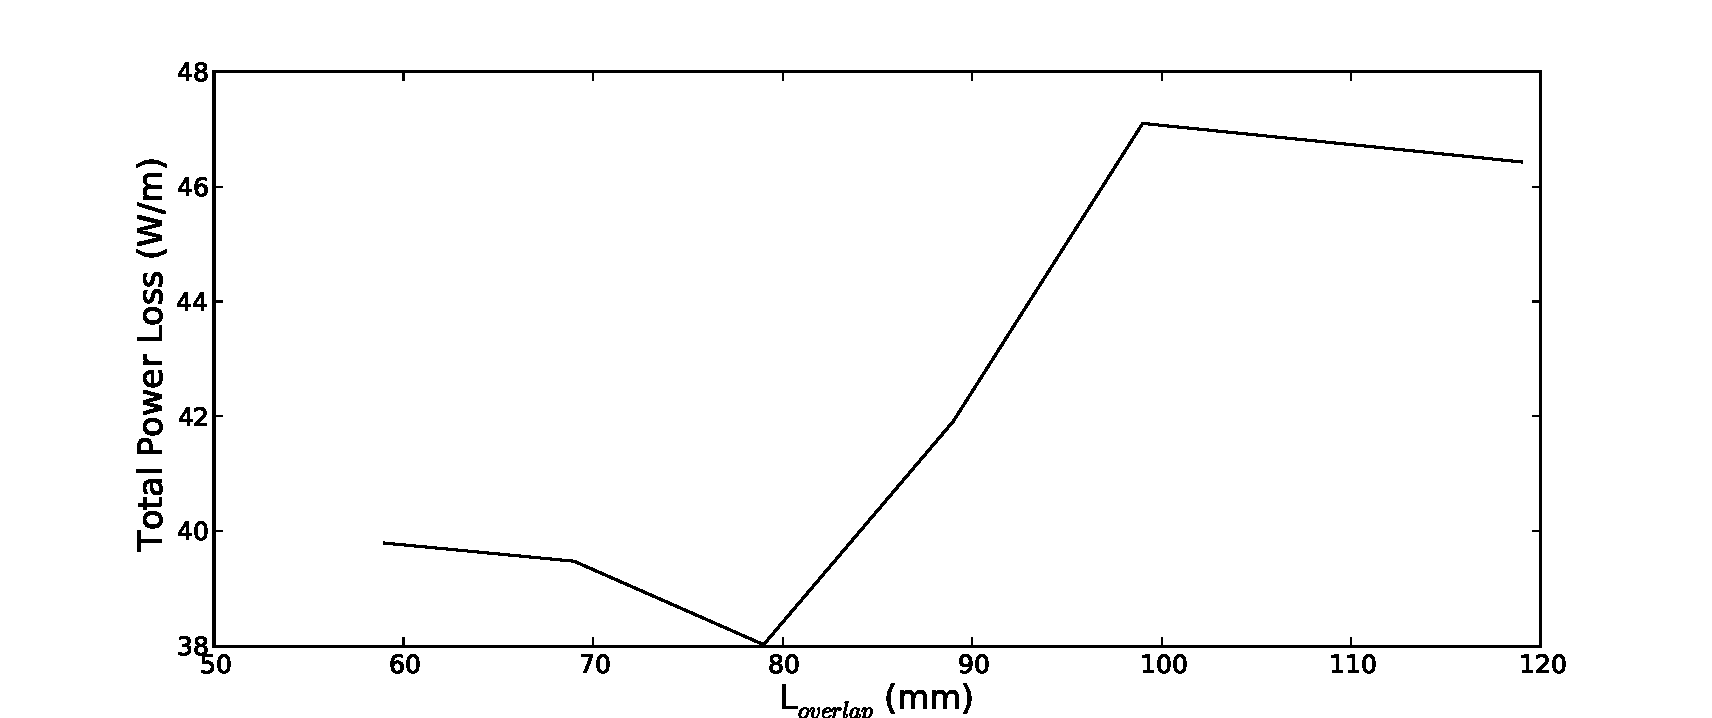
\includegraphics[width=0.55\textwidth]{heatingOverlapFull.pdf}
\caption{Power loss for various overlap lengths with Post-LS1 parameters}
\label{fig:powLossTotal}
\end{figure}

\begin{itemize}
\item{The power loss for various values of $L_{overlap}$ is shown in Fig.~\ref{fig:powLossTotal}, assuming Post-LS1 parameters for the LHC (see Table.~1). It can be seen that the minimum occurs in the region of 70mm-80mm, giving a reduction of some 20\% over the 107mm as is the case for the current design.}
\item{This power loss corresponds to 140W/m with HL-LHC parameters, close to that calculated for the non-conforming MKI8D - in this case the temperature of the ferrite yoke would still be uncomfortably close to the Curie temperature during operation indicating improved cooling must also be considered [3]. A prototype is intended to be installed in the LHC for testing prior to LS2}
\end{itemize}


\end{block}

\vfill
\begin{block}{References}
\begin{enumerate}
\item{\small{M.J. Barnes \emph{et al}., \emph{Upgrade of the LHC Injection Kicker Magnets}, IPAC2013, MOPWA030}}
\item{\small{H. Day \emph{et al}., \emph{Beam Coupling Impedance of the New Beam Screen of the LHC Injection Kickers}, IPAC2014, TUPRI030}}
\item{\small{M.J. Barnes \emph{et al}., \emph{Cooling of the LHC Injection Kicker Magnet Ferrite Yoke: Measurements and Future Proposals}, IPAC2014, MOPME075}}
\end{enumerate}
\end{block}


\vfill

          }
          % ---------------------------------------------------------%
          % end the column
        \end{minipage}
      \end{beamercolorbox}
    \end{column}
    % ---------------------------------------------------------%
    % end the column
  \end{columns}

  %\tiny\hfill\textcolor{ta2gray}{Created with \LaTeX \texttt{beamerposter}  \url{http://www-i6.informatik.rwth-aachen.de/~dreuw/latexbeamerposter.php}}
%  \tiny\hfill{Created with \LaTeX \texttt{beamerposter}  \url{http://www-i6.informatik.rwth-aachen.de/~dreuw/latexbeamerposter.php} \hskip1em}
\end{frame}
\end{document}


%%%%%%%%%%%%%%%%%%%%%%%%%%%%%%%%%%%%%%%%%%%%%%%%%%%%%%%%%%%%%%%%%%%%%%%%%%%%%%%%%%%%%%%%%%%%%%%%%%%%
%%% Local Variables: 
%%% mode: latex
%%% TeX-PDF-mode: t
%%% End:
